En resumen, en nuestra prueba de calibración de los SiPM tenemos una caja que actuará como jaula de faraday, con temperatura y humedad controlada y apantallada en lo posible de la luz del exterior. 

En su interior tendremos un diodo LED que emite fotones a $\lambda=435~\nm$, un SiPM, el cual emitirá un pulso de intensidad cada vez que detecte uno o más de estos fotones con cada uno de sus pixels y una tarjeta que convertirá este pulso de intensidad en un pulso de voltaje. Finalmente llevamos este pulso de voltaje a un osciloscopio (marca TELEDYNE LECROY, modelo WwaveRunner 625Zi) para poder ser analizado. 

Una vez en el osciloscopio, la señal que recibíamos cuando se encendía el diodo LED será similar a la de la señal superior de la figura 13 (amarilla)~\cite{inftec}, el la cual se a activado el modo persistencia del osciloscopio con el objetivo de comparar señales de distintas alturas. Estas señales corresponden a distinto número de pixels activados en cada instante de tiempo ya que, como hemos dicho anteriormente, la señal de salida del sistema es la suma de las señales de cada pixel que se ha activado. Esta se encuentra superpuesta a la señal de sincronización del generador de señales (verde) que nos muestra cuando se ha encendido el diodo LED y que, por tanto, actua como trigger.

El objetivo ahora es calcular la ganancia del sistema. Dado que únicamente existen dos ganancias en el sistema (SiPM y tarjeta) y hemos medido la ganancia de la tarjeta en la sección anterior, determinando la ganancia total podremos determinar de forma aproximada la ganancia del SiPM. 

\begin{equation}
G_{tot}=G_{SiPM} \cdotp G_{card} \longrightarrow G_{SiPM} = \frac{G_{tot}}{G_{card}}
\label{ganancias}
\end{equation}

Para medir la ganancia total simplemente realizamos una integral del area de cada uno de los pulsos de salida del sistema y conservamos el resultado en un histograma. De esta forma lo que estamos consiguiendo es un histograma de las cargas de los pulsos. La ventana temporal sobre la que se integra es aproximadamente una división, que equivale a $500~\ns$. Esta se ajusta con bastante precisión al pulso, algo muy importante para evitar la introducción de background.

Dado que idealmente el pulso de cada pixel es igual, el histograma que estamos obteniendo deberían ser deltas de dirac equiespaciadas. Sin embargo hay que tener en cuenta que la cascada que produce cada uno de estos fotones detectados en cada pixel esta sometido a fluctuaciones estadísticas. Además los propios instrumentos de medidas empleados tienen una incertidumbre inherente. Hay que tener en cuenta que tambień tenemos distintas fuentes de background, como dark counts (ruido térmico), fotones de luz del exterior, etc. 

Como resultado de todo esto, lo que obtendremos seran un conjunto de gaussianas equiespaciadas. En la figura 13 inferior puede verse el resultado de una toma de datos de 25000 eventos a 25 grados, 60\% de humedad y $V_{ov}=3V$

\begin{figure}[hbtp]
 \centering
 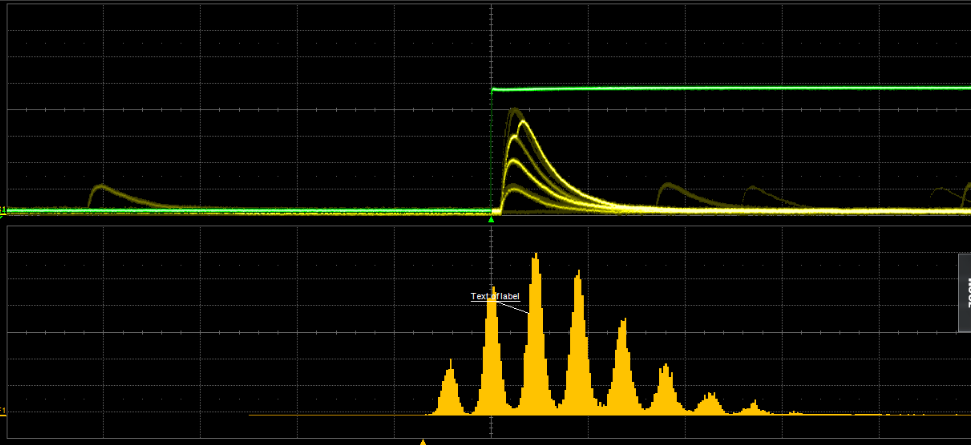
\includegraphics[scale=0.4]{Analisis.png}
 \caption{Análisis\label{analisis}}
 \end{figure}

Donde cada uno de estos picos corresponde a la carga de sucesivos número de pixels activados (uno, dos, etc.). El primer pico no debe tenerse en cuenta en el análisis ya que este corresponde al pedestal (cero pixels activados). Su origen es debido a la existencia de las cuentas ocuras.
 
Ahora únicamente desarrollamos una macro en ROOT (programa de análisis de datos desarrollado por el CERN) que, utilizando la librería TSpectrum (librería especialmente diseñada para el análisis de histograma) nos permita obtener la ganancia del sistema. Su forma de proceder es la siguiente:
\begin{enumerate}
\item {} Primero la macro lee el fichero de datos, los guarda en una variable de tipo histograma y los representa. La macro termina de leer el fichero cuando no encuentra más valores.

\item {} A continuación, a partir de una función de la librería TSpectrum, busca en este histograma y devuelve el número de gaussianas que ha encontrado y su posición.

\item {} Ahora ajusta todos los datos del histograma a una recta y solo se queda con las gaussianas, cuya norma sobrepasa en altura a esta recta. El objetivo de este paso es que, en casos muy concretos (temperatura alta o luz del laboratorio encendida) tenemos mucho ruido y, aparece un fondo el cual, el programa ajusta a una gaussiana y, por extensión, calcula la ganancia de manera incorrecta. Un ejemplo de esto se muestra en la figura 14.

\begin{figure}[hbtp]
\centering
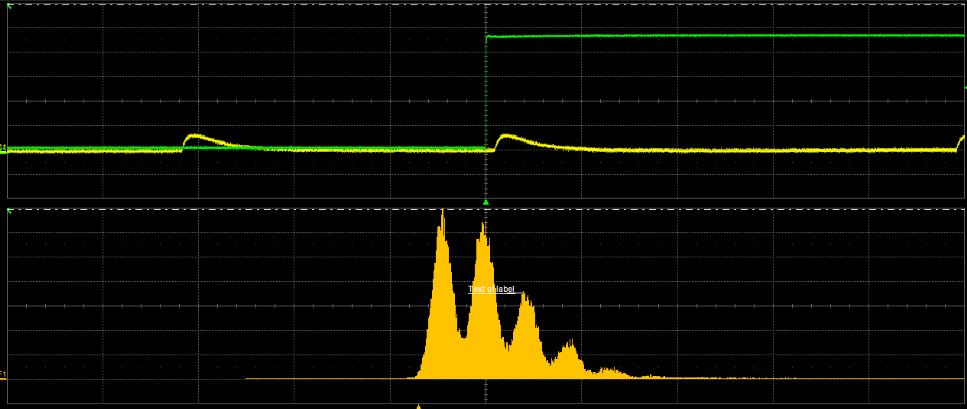
\includegraphics[scale=0.4]{fondogaussiano.png}
\caption{Espectro con mucho fondo\label{fondogrande}}
\end{figure}

\item {} Seguidamente, ajustamos el espectro a una recta mas una suma de n gaussianas, donde n es el número de gaussianas que superan la recta (calculado en el paso anterior). La necesidad de utilizar una recta es debido a que siempre vamos a tener dark counts y otro tipo de bakcground que se verán reflejados en una linea base en el histograma como puede verse en la figura \ref{analisis}. Podemos apreciar en la figura 15 que el ajuste (linea roja) es relativamente bueno. Para poder ver hasta que punto nuestro ajuste es aceptable aplicamos el test $\chi^2$, donde se ha obtenido un resultado de $\frac{\chi^2}{ndf}=\frac{1276}{223}\approx 5.72$. Vemos que efectivamente el ajuste se realizado con gran precisión.

\begin{figure}[hbtp]
\centering
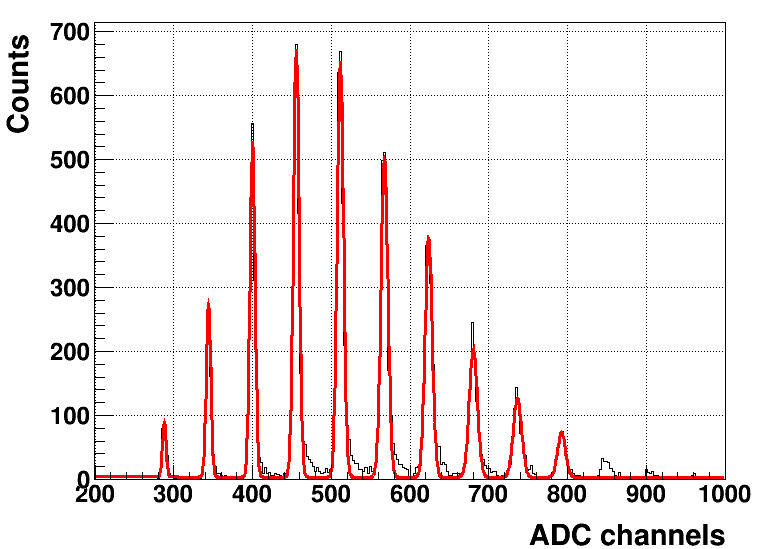
\includegraphics[scale=0.4]{AjusteEspectro1.png}
\caption{ Ajuste de la macro de ROOT sobre un espectro\label{Root}}
\end{figure}

\item {} Dado que se ha observado que, aun con el tercer paso, existen situaciones límites en que el background sigue superando esta recta, se ha incluido un paso en la macro en la cual se acepta por teclado uno a uno los picos que serán utilizados en el análisis. Además la macro calcula la resolución de cada gaussiana y la resolución total, obtenida a partir de la suma cuadrática de la resolución de cada gaussiana. Los valores habitualmente encontrados en los análisis se encuentran sobre 1.5\% y 5\% respectivamente, valores más que aceptables.

\item {} Finalmente la macro los ordena según su posición en el espectro y calcula la ganancia por dos caminos:
	\begin{enumerate}

	\item {} Por un lado se ha calculado la distancia promedio entre sucesivas gaussianas del espectro~\cite{Hueso}.
	\begin{equation} 
	Q = G N_\gamma + Q_0 \longrightarrow \Delta Q= Q_{N_\gamma} - Q_{N_\gamma -1}=G N_\gamma+ Q_0 - G(N_		\gamma -1) - Q_0 = G
	\label{gananciametodo1}
	\end{equation}
	Podemos observar que este cálculo corresponde a la ganancia. Hay que tener en cuenta que se han empleados factores de conversión para convertir la posición del pico (inicialmente en unidades de	tensión, V) en unidades de carga (coulomb). En concreto se ha utilizado el factor $\frac{1}{eR}$, donde R es la resistencia del osciloscopio, 50 $\Omega$ y e es la carga del electrón.
	
	\item {} Por otro lado se ha ajustado a una recta las posiciones horizontales de estas gaussianas en el 	espectro frente a el número de pixels. Esto nos da la siguiente ecuación~\cite{Hueso}:
	\begin{equation}
	Centro\_pico(V) = GeRN_\gamma + k_0
	\label{gananciametodo2}
	\end{equation}
	Donde R y e significan lo mismo. Vemos por tanto que apartir del valor de la pendiente podemos obtener	el valor de la ganancia. La figura 16 muestra un ejemplo de ajuste entre posiciones de gaussianas y número de pixels para el caso de 25 grados, humedad de 45\% y $V_{ov}=3V$. Podemos observar que existe	un acuerdo excelente, algo que ocurria prácticamente en la totalidad de los casos. Este gráfico presenta barras de error pero no son apreciables a esta escala.
		
	\begin{figure}[hbtp]
		\centering
		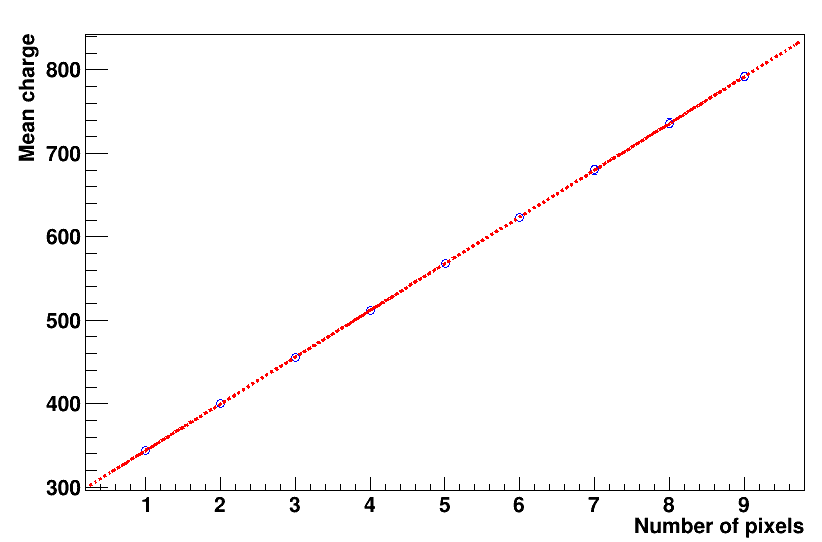
\includegraphics[scale=0.4]{FitPosicionPixels.png}
		\caption{Ajuste carga de las señales del SiPM frente a nº de pixels encendidos\label{ajuste}}
		\end{figure}
			
	\end{enumerate}
	
Para este caso concreto las ganancias obtenidas por los dos caminos anteriores son respectivamentente:
\begin{equation}
G_1= 6.38938 \cdot 10^8 \pm 2.15953 \cdot 10^8
\label{gananciatotalmetodo1} 
\end{equation}
\begin{equation}
G_2=7.18235 \cdot 10^8 \pm 6.88392 \cdot 10^6
\label{gananciatotalmetodo2}
\end{equation}
Por extensión, las ganancias del SiPM calculadas por cada camino son (aproximadamente)$\eqref{ganancias}$: 
\begin{equation}
G_1= 5.80853 \cdot 10^6 \pm 1.96321 \cdot 10^6
\label{gananciaSiPMmetodo1}
\end{equation}
\begin{equation}
G_2= 6.52941 \cdot 10^6 \pm 6.258 \cdot 10^4
\label{gananciaSiPMmetodo2}
\end{equation}

donde los errores se han obtenido por propagación. Si comparamos con la literatura~\cite{datasheet SiPM} podemos observar que ambos valores son bastante aceptables con errores relativos de:

\begin{equation}
\sigma_{rel1} \approx 0.0319 = 3.19\%; \qquad \sigma_{rel2} \approx 0.0882 = 8,82\%
\label{erroresgananciasSiPM}
\end{equation}


Dado que, en la practica, las gaussianas no estan perfectamente equiespaciadas debido a errores e incertidumbres consideraremos como más fiable el segundo método ya que se trata de un método más formal, a pesar de tener un error relativo mayor.

Nuevamente se ha aplicado el test $\chi^2$ con el objetivo de comprobar la calidad de nuestro ajuste. Se ha obtenido un resultado de $\frac{\chi^2}{ndf}=\frac{0.05452}{7}\approx 0.008$. Podemos apreciar que ahora hemos obtenido un valor bastante por debajo de la unidad. Este, probablemente, es debido a que se han sobreestimado los errores de las medidas (calculados a partir de las sigmas de las gaussianas del ajuste de la figura $\ref{Root}$).

\end{enumerate}